% ==========================================================================
%  Where does the back wave go?  --  loudspeaker enclosures on one 16:9 landscape poster
%  Same palette, type and boxes as the Ten Commandments poster.
%  Compile: just
% ==========================================================================
\RequirePackage{fix-cm}
\documentclass{article}
\usepackage[paperwidth=1067mm,paperheight=600mm,left=13mm,right=13mm,top=8mm,bottom=10mm]{geometry}
\usepackage[utf8]{inputenc}
\usepackage[T1]{fontenc}
\usepackage[sc]{mathpazo}          % Palatino text + math
\linespread{1.05}
\usepackage{amsmath,amssymb,bm}
\usepackage{xcolor}
\usepackage{tikz}
\usetikzlibrary{arrows.meta,calc,patterns}
\usepackage{pgfplots}
\pgfplotsset{compat=1.16}
\usepackage[most]{tcolorbox}
\usepackage[hidelinks]{hyperref}

\pagestyle{empty}
\setlength{\parindent}{0pt}

% ---------------- palette ----------------
\definecolor{paper}{HTML}{F8F5EE}
\definecolor{ink}{HTML}{1E2430}
\definecolor{accent}{HTML}{1F4E79}
\definecolor{accentlt}{HTML}{6E93B5}
\definecolor{trap}{HTML}{9A3B2E}
\definecolor{muted}{HTML}{6B7280}
\definecolor{rule}{HTML}{B9C6D3}
\definecolor{good}{HTML}{3C7A4A}
\definecolor{steel}{HTML}{D9DEE4}
\pagecolor{paper}
\color{ink}

\newcommand{\repourl}{https://github.com/samo4/ee-posters}

% ---------------- sizes ----------------
\renewcommand{\normalsize}{\fontsize{17}{21}\selectfont}
\renewcommand{\small}{\fontsize{14}{17}\selectfont}
\renewcommand{\footnotesize}{\fontsize{12.5}{15}\selectfont}
\newcommand{\eqsize}{\fontsize{19}{23}\selectfont}
\normalsize

\newcommand{\setdisplay}{%
  \setlength{\abovedisplayskip}{3pt}\setlength{\belowdisplayskip}{3pt}%
  \setlength{\abovedisplayshortskip}{3pt}\setlength{\belowdisplayshortskip}{3pt}}

% ---------------- equation group: a thin box holding equations that belong together
\newtcolorbox{eqgroup}[1][]{%
  enhanced, colback=white, colframe=rule, boxrule=0.7pt, arc=2.5mm,
  left=6pt, right=6pt, top=5pt, bottom=2pt, before skip=8pt, after skip=2pt,
  fontupper=\eqsize, before upper={\setdisplay},
  title={#1}, fonttitle=\footnotesize\scshape, coltitle=muted,
  attach boxed title to top left={xshift=4mm, yshift=-\tcboxedtitleheight/2},
  boxed title style={colback=white, colframe=white, boxrule=0pt, arc=0pt,
                     left=3pt, right=3pt, top=0pt, bottom=0pt}}
% short prose inside a box
\newcommand{\note}[1]{{\small\color{muted}#1\par}}

\newcommand{\trapicon}{\tikz[baseline=-0.15em]{%
  \fill[trap, rounded corners=1.2pt] (0,-0.12em) -- (1.15em,-0.12em) -- (0.575em,0.92em) -- cycle;
  \node[white, font=\bfseries\fontsize{11}{11}\selectfont, inner sep=0pt] at (0.575em,0.27em) {!};}}
\newcommand{\trap}[1]{{\centering\fontsize{14.5}{17.5}\selectfont\itshape\color{trap}#1\par}}

% ---------------- enclosure box ----------------
% [#1] extra options, #2 name, #3 the maxim, #4 where you meet it (sits on the bottom border)
\newtcolorbox{enclosure}[4][]{%
  enhanced, colback=white, colframe=accent, boxrule=1.4pt, arc=4mm,
  left=8pt, right=8pt, top=3pt, bottom=12pt,
  title={%
    \begin{tikzpicture}[baseline=(n.base)]
      \node[rounded corners=5mm, fill=white, text=accent, minimum height=11mm, inner xsep=3mm, inner ysep=0pt,
            font=\fontsize{23}{23}\selectfont\bfseries] (n) {#2};
    \end{tikzpicture}\par\vspace{1.5mm}
    {\fontsize{20}{24}\selectfont\bfseries\itshape #3}},
  colbacktitle=accent, coltitle=white,
  toptitle=4pt, bottomtitle=4pt, lefttitle=8pt, righttitle=8pt,
  segmentation hidden, space to upper, middle=1pt,
  overlay={\node[fill=white, draw=accent, line width=1.4pt, rounded corners=2.5mm, text width=140mm, align=center,
                 inner xsep=9pt, inner ysep=5pt, font=\small, text=ink, anchor=center]
                 at (frame.south) {#4};},
  #1}

% the cross-section (left) and its response (right)
\newcommand{\figs}[2]{%
  \begin{minipage}[c]{0.36\linewidth}\centering #1\end{minipage}\hfill
  \begin{minipage}[c]{0.63\linewidth}\centering #2\end{minipage}\par}

% ---------------- cross-sections ----------------
\tikzset{section/.style={x=10.5mm, y=10.5mm, line cap=round},
         wall/.style={ink, line width=2.4pt},
         frontwave/.style={accent, line width=1.8pt, -{Latex[length=2.6mm]}},
         backwave/.style={trap, line width=1.8pt, -{Latex[length=2.6mm]}},
         portwave/.style={good, line width=1.8pt, -{Latex[length=2.6mm]}},
         stuffing/.style={pattern=dots, pattern color=muted!70},
         lbl/.style={font=\small, text=ink}}
% a driver whose cone opens towards +x at #2, turned by #1 degrees; magnet behind
\newcommand{\driver}[2][0]{\begin{scope}[shift={#2}, rotate=#1]
  \fill[ink] (-0.75,-0.3) rectangle (-0.45,0.3);
  \draw[ink, line width=1.2pt, fill=steel] (-0.45,-0.2) -- (0,-0.8) -- (0,0.8) -- (-0.45,0.2) -- cycle;
  \end{scope}}
% a passive radiator: a cone with no motor
\newcommand{\radiator}[1]{\begin{scope}[shift={#1}]
  \draw[ink, line width=1.2pt, fill=white] (-0.45,-0.2) -- (0,-0.8) -- (0,0.8) -- (-0.45,0.2) -- cycle;
  \fill[ink] (-0.5,-0.2) rectangle (-0.42,0.2);
  \end{scope}}

% ---------------- responses: level in dB over f/f_0 ----------------
\pgfplotsset{resp/.style={
  scale only axis, width=84mm, height=72mm, xmin=0.1, xmax=10, ymin=-36, ymax=6,
  axis x line=bottom, axis y line=left, axis line style={-{Latex[length=3mm]}, thick},
  tick style={draw=none}, ticklabel style={font=\small}, label style={font=\normalsize},
  ytick={0,-24}, yticklabels={$0$\,dB,$-24$},
  every axis x label/.style={at={(axis description cs:1,0)}, anchor=west, xshift=1mm},
  xlabel={$f$}, samples=240, domain=0.1:10, restrict y to domain=-90:30,
  every axis plot/.append style={line width=1.8pt}}}
% second-order high-pass and low-pass magnitude, x = f/f_0
\pgfmathdeclarefunction{hp}{2}{\pgfmathparse{#1^2/sqrt((1-#1^2)^2+(#1/#2)^2)}}
\pgfmathdeclarefunction{lp}{2}{\pgfmathparse{1/sqrt((1-#1^2)^2+(#1/#2)^2)}}
% impedance magnitude over f/f_0: every resonance shows up as a peak
\pgfplotsset{imp/.style={
  scale only axis, width=145mm, height=26mm, xmin=0.1, xmax=10, ymin=0, ymax=9.5,
  axis x line=bottom, axis y line=left, axis line style={-{Latex[length=3mm]}, thick},
  tick style={draw=none}, ticklabel style={font=\small}, label style={font=\normalsize},
  ytick={1}, yticklabels={$R_e$}, ylabel={$|Z|$},
  every axis y label/.style={at={(axis description cs:0,1)}, anchor=south west},
  every axis x label/.style={at={(axis description cs:1,0)}, anchor=west, xshift=1mm},
  xlabel={$f$}, samples=300, domain=0.1:10}}
% a resonance peak in |Z|: #1 height, #2 frequency, #3 sharpness
\pgfmathdeclarefunction{zpk}{4}{\pgfmathparse{#2/sqrt(1+#4*(#1/#3-#3/#1)^2)}}
% #1 axis options, #2 |Z|(x) on top of R_e and the voice coil's inductance
\newcommand{\impedance}[2][]{\par\vspace{2mm}{\centering
  \begin{tikzpicture}\begin{semilogxaxis}[imp, #1]
    \draw[muted, dashed, line width=0.8pt] (axis cs:0.1,1) -- (axis cs:10,1);
    \addplot[ink, line width=1.6pt] {1+0.25*x+#2};
  \end{semilogxaxis}\end{tikzpicture}\par}}
\newcommand{\zerodb}{\draw[muted, dashed, line width=0.8pt] (axis cs:0.1,0) -- (axis cs:10,0);}
\newcommand{\slope}[3]{\node[font=\small, text=muted, anchor=west] at (axis cs:#1,#2) {#3};}

% a column that fills the page height; \vfill between blocks spreads them out
\newenvironment{pagecol}[1]{\begin{minipage}[t][\dimexpr\textheight-\topskip\relax][s]{#1}\vspace{0pt}}{\end{minipage}}

\begin{document}
\noindent
% ===================================================================== LEFT: title, the driver, the iron law
\begin{pagecol}{0.255\linewidth}
% gutter notes, read top to bottom along the left and right page edges
\begin{tikzpicture}[remember picture, overlay]
  \node[rotate=-90, anchor=center, text=muted, font=\fontsize{14}{17}\selectfont\itshape]
    at ($(current page.east)+(-6.3mm,0mm)$)
    {No woofers were bottomed out in the making of this poster.\quad
     \upshape\href{\repourl}{\color{accent}\repourl}};
  \node[rotate=-90, anchor=center, text=muted, font=\fontsize{17}{20}\selectfont\itshape]
    at ($(current page.west)+(6.3mm,0mm)$)
    {The room is the last enclosure, and the one you did not design.};
\end{tikzpicture}%
{\fontsize{28}{32}\selectfont\scshape\color{muted} Loudspeaker enclosures, or:}\\[2mm]
{\fontsize{72}{76}\selectfont\bfseries Where does\\ the back wave go?}\par
\vspace{4mm}
{\color{accent}\rule{\linewidth}{2.5pt}}\par
\vspace{4mm}
{\fontsize{23}{28}\selectfont\color{muted}\itshape
 The back of the cone sings as loud as the front,\\ in antiphase. Every box is an argument with it.\\[1mm]
 \upshape\bfseries\color{trap} Small, deep, loud: pick two.}\par
\vfill
{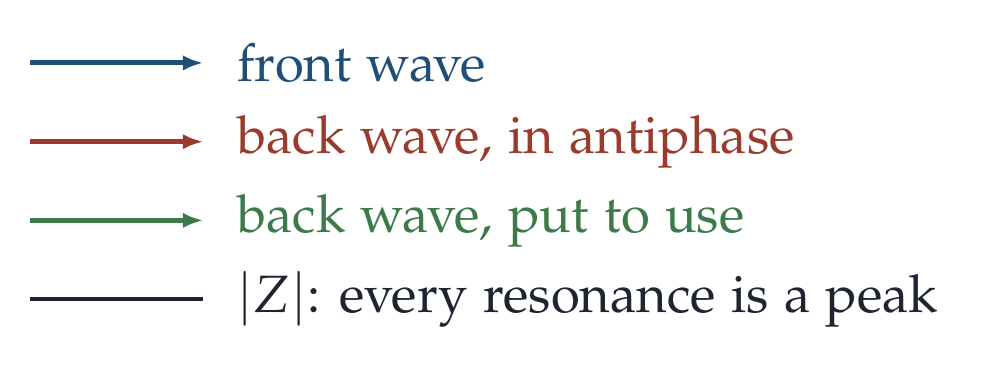
\begin{tikzpicture}[x=1mm, y=1mm, font=\fontsize{19}{23}\selectfont, every node/.style={anchor=west}]
  \draw[frontwave] (0,30) -- (22,30) node[right=2mm] {front wave};
  \draw[backwave] (0,20) -- (22,20) node[right=2mm] {back wave, in antiphase};
  \draw[portwave] (0,10) -- (22,10) node[right=2mm] {back wave, put to use};
  \draw[ink, line width=1.6pt] (0,0) -- (22,0) node[right=2mm] {$|Z|$: every resonance is a peak};
\end{tikzpicture}\par}
\vfill
\begin{tcolorbox}[enhanced, colback=white, colframe=ink, boxrule=1.6pt, arc=4mm, left=10pt, right=10pt, top=4pt, bottom=8pt,
  title={\fontsize{30}{34}\selectfont\bfseries The driver}, colbacktitle=ink, coltitle=white,
  toptitle=4pt, bottomtitle=4pt, lefttitle=10pt]
  \begin{eqgroup}[Thiele--Small: a mass on a spring, damped twice]
  \[ f_s=\frac{1}{2\pi\sqrt{M_{ms}C_{ms}}}\qquad Q_{ts}=\frac{Q_{es}\,Q_{ms}}{Q_{es}+Q_{ms}} \]
  \[ V_{as}=\rho_0c^2S_d^2\,C_{ms} \]
  \note{$V_{as}$: the volume of air as stiff as the suspension. Every box below is measured against it.}
  \end{eqgroup}
  \begin{eqgroup}[A piston in a wall radiates its acceleration]
  \[ p(r)=\frac{\rho_0\,S_d\,\ddot x}{2\pi r} \]
  \note{Flat response means constant acceleration, so excursion $x=\ddot x/\omega^2$ grows fourfold for every octave down.}
  \end{eqgroup}
  \vspace{3mm}
  {\centering
  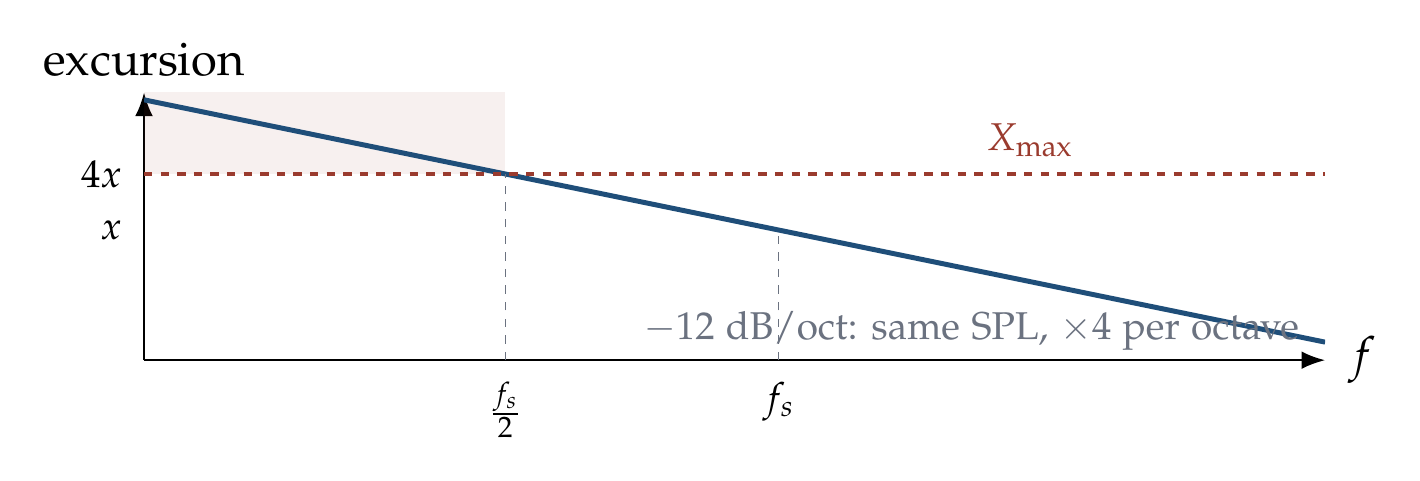
\begin{tikzpicture}
  \begin{loglogaxis}[scale only axis, width=150mm, height=34mm, xmin=0.2, xmax=4, ymin=0.04, ymax=30,
      axis x line=bottom, axis y line=left, axis line style={-{Latex[length=3mm]}, thick}, tick style={draw=none},
      xtick={0.5,1}, xticklabels={$\tfrac{f_s}{2}$,$f_s$}, ytick={1,4}, yticklabels={$x$,$4x$}, ticklabel style={font=\small},
      xlabel={$f$}, ylabel={excursion}, label style={font=\normalsize},
      every axis x label/.style={at={(axis description cs:1,0)}, anchor=west, xshift=1mm},
      every axis y label/.style={at={(axis description cs:0,1)}, anchor=south}]
    \fill[trap, opacity=0.08] (axis cs:0.2,4) rectangle (axis cs:0.5,30);
    \addplot[accent, line width=1.8pt, domain=0.2:4, samples=40] {1/x^2};
    \draw[trap, dashed, line width=1.2pt] (axis cs:0.2,4) -- (axis cs:4,4) node[pos=0.75, above, font=\small] {$X_\text{max}$};
    \draw[muted, dashed, thin] (axis cs:0.5,0.04) -- (axis cs:0.5,4) (axis cs:1,0.04) -- (axis cs:1,1);
    \node[font=\small, text=muted, anchor=north east] at (axis cs:3.9,0.2) {$-12$ dB/oct: same SPL, $\times4$ per octave};
  \end{loglogaxis}
  \end{tikzpicture}\par}
  \begin{eqgroup}[Efficiency, and why it is an iron law]
  \[ \eta_0=\frac{4\pi^2}{c^3}\,\frac{f_s^3\,V_{as}}{Q_{es}}\qquad \eta_0=k_\eta\,f_3^3\,V_b \]
  \[ \mathrm{EBP}=\frac{f_s}{Q_{es}}:\quad\lesssim50\ \text{closed},\ \ \gtrsim100\ \text{vented} \]
  \note{Hofmann: for a given alignment, efficiency is fixed by $f_3^3V_b$. An octave deeper in the same box costs 9\,dB.}
  \end{eqgroup}
  \vspace{4mm}
  {\centering
  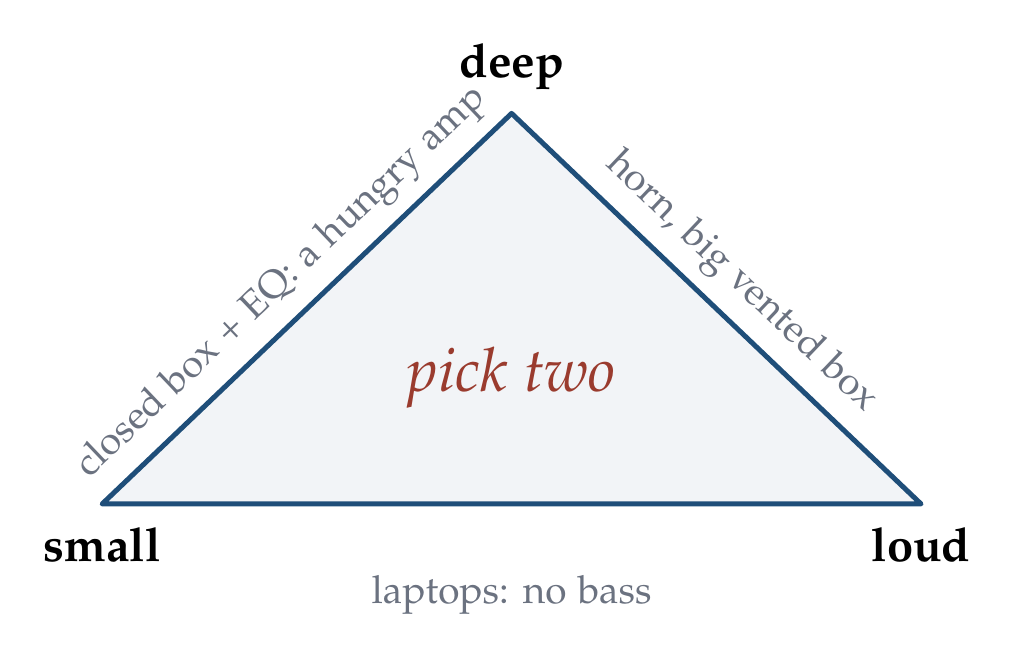
\begin{tikzpicture}[x=0.8mm, y=0.8mm, font=\normalsize]
    \coordinate (S) at (0,0); \coordinate (L) at (130,0); \coordinate (D) at (65,62);
    \fill[accent!6] (S) -- (L) -- (D) -- cycle;
    \draw[accent, line width=1.8pt, line join=round] (S) -- (L) -- (D) -- cycle;
    \node[below=1mm, font=\normalsize\bfseries] at (S) {small};
    \node[below=1mm, font=\normalsize\bfseries] at (L) {loud};
    \node[above=1mm, font=\normalsize\bfseries] at (D) {deep};
    \node[font=\fontsize{22}{26}\selectfont\itshape\color{trap}] at (65,20) {pick two};
    \node[font=\small, text=muted, rotate=43.6, above] at ($(S)!0.5!(D)$) {closed box + EQ: a hungry amp};
    \node[font=\small, text=muted, rotate=-43.6, above] at ($(L)!0.5!(D)$) {horn, big vented box};
    \node[font=\small, text=muted, below=7mm] at ($(S)!0.5!(L)$) {laptops: no bass};
  \end{tikzpicture}\par}
\end{tcolorbox}
\end{pagecol}\hfill
% ===================================================================== RIGHT: eight enclosures
\begin{minipage}[t]{0.73\linewidth}\vspace{0pt}
\begin{tcbraster}[raster columns=4, raster equal height=rows, raster column skip=6mm, raster row skip=16mm,
                  raster force size=false]
% ---------------------------------------------------------------- infinite baffle
\begin{enclosure}[height=268mm, valign upper=center]{Infinite baffle}{Let the back wave go somewhere else.}%
  {Ceiling and in-wall speakers, car rear decks.}
\figs{%
  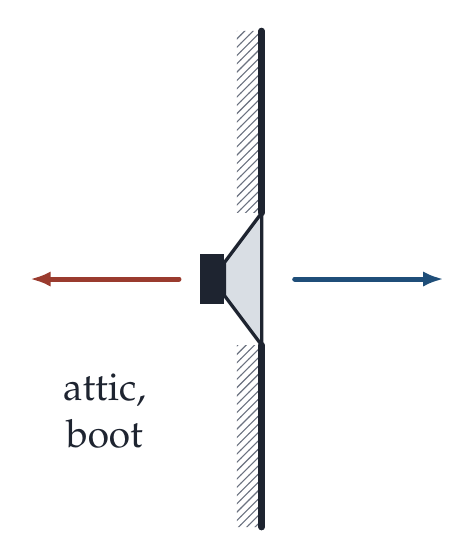
\begin{tikzpicture}[section]
    \fill[pattern=north east lines, pattern color=muted] (-0.3,0.8) rectangle (0,3) (-0.3,-3) rectangle (0,-0.8);
    \draw[wall] (0,3) -- (0,0.8) (0,-0.8) -- (0,-3);
    \driver{(0,0)}
    \draw[frontwave] (0.4,0) -- (2.2,0);
    \draw[backwave] (-1,0) -- (-2.8,0);
    \node[lbl, align=center] at (-1.9,-1.6) {attic,\\ boot};
  \end{tikzpicture}}{%
  \begin{tikzpicture}
  \begin{semilogxaxis}[resp, xtick={1}, xticklabels={$f_s$}]
    \zerodb
    \addplot[accent] {20*log10(hp(x,0.5))};
    \slope{0.12}{-30}{$-12$ dB/oct}
  \end{semilogxaxis}
  \end{tikzpicture}}
\impedance[xtick={1}, xticklabels={$f_s$}]{zpk(x,7,1,9)}
\begin{eqgroup}[The driver's own high-pass, nothing added]
\[ H(s)=\frac{s^2}{s^2+s\,\omega_s/Q_{ts}+\omega_s^2} \]
\note{Holds while $V_\text{back}\gg V_{as}$: at $\alpha=V_{as}/V_\text{back}=0.1$, $f_s$ already moves 5\,\%.}
\end{eqgroup}
\tcblower
\trap{\textbf{An infinite baffle is a wall, not a plank.} A finite one is an open baffle.}
\end{enclosure}
% ---------------------------------------------------------------- open baffle
\begin{enclosure}[height=268mm, valign upper=center]{Open baffle}{Let the back wave meet the front, and cancel.}%
  {Electrostatic and ribbon panels, open-back guitar cabinets.}
\figs{%
  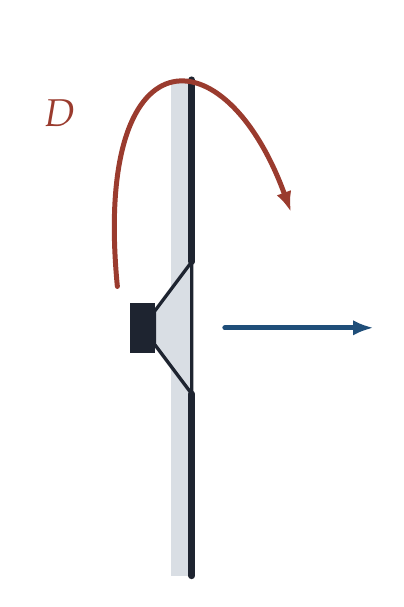
\begin{tikzpicture}[section]
    \fill[steel] (-0.25,-3) rectangle (0,3); \draw[wall] (0,3) -- (0,0.8) (0,-0.8) -- (0,-3);
    \driver{(0,0)}
    \draw[frontwave] (0.4,0) -- (2.2,0);
    \draw[backwave] (-0.9,0.5) .. controls (-1.2,3.6) and (0.4,3.6) .. (1.2,1.4);
    \node[lbl, text=trap] at (-1.6,2.6) {$D$};
  \end{tikzpicture}}{%
  \begin{tikzpicture}
  \begin{semilogxaxis}[resp, xtick={1,3}, xticklabels={$f_s$,$\tfrac{c}{2D}$}]
    \zerodb
    \addplot[accent] {20*log10(hp(x,0.5)*(x/3)/sqrt(1+(x/3)^2))};
    \addplot[muted, dashed, line width=1.2pt] {20*log10(hp(x,0.5))};
    \slope{0.2}{-30}{$-18$ dB/oct}
  \end{semilogxaxis}
  \end{tikzpicture}}
\impedance[xtick={1}, xticklabels={$f_s$}]{zpk(x,7,1,9)}
\begin{eqgroup}[Front and back, a path $D$ apart]
\[ |p_\text{dipole}|=2\,|p|\,\Bigl|\sin\frac{\pi fD}{c}\Bigr| \]
\[ f_\text{peak}=\frac{c}{2D}\qquad\text{\small\color{muted}($D=0.5$\,m: 343\,Hz)} \]
\note{Below the peak it loses 6\,dB/oct on top of the driver's 12. Polar pattern: a figure eight, $\cos\theta$.}
\end{eqgroup}
\tcblower
\trap{\textbf{Bass from a dipole needs a door-sized baffle,} or excursion the driver does not have.}
\end{enclosure}
% ---------------------------------------------------------------- closed box
\begin{enclosure}[height=268mm, valign upper=center]{Closed box}{Trap the back wave; the air becomes a spring.}%
  {Studio monitors, sealed subwoofers; the AR-1, 1954.}
\figs{%
  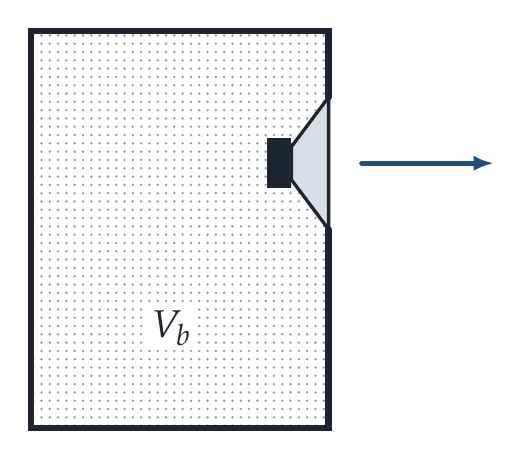
\begin{tikzpicture}[section]
    \fill[stuffing] (-3.6,-2.4) rectangle (0,2.4);
    \draw[wall] (0,1.6) -- (0,2.4) -- (-3.6,2.4) -- (-3.6,-2.4) -- (0,-2.4) -- (0,0);
    \driver{(0,0.8)}
    \draw[frontwave] (0.4,0.8) -- (2,0.8);
    \node[lbl, fill=white, inner sep=1.5pt] at (-1.9,-1.2) {$V_b$};
  \end{tikzpicture}}{%
  \begin{tikzpicture}
  \begin{semilogxaxis}[resp, xtick={1}, xticklabels={$f_c$}]
    \zerodb
    \addplot[trap, line width=1.2pt] {20*log10(hp(x,1.4))};
    \addplot[muted, dashed, line width=1.2pt] {20*log10(hp(x,0.5))};
    \addplot[accent] {20*log10(hp(x,0.707))};
    \node[font=\small, text=trap, anchor=south] at (axis cs:1.1,3) {$1.4$};
    \node[font=\small, text=accent, anchor=west] at (axis cs:2,-5) {$Q_{tc}=0.707$};
    \slope{0.12}{-30}{$-12$ dB/oct}
  \end{semilogxaxis}
  \end{tikzpicture}}
\impedance[xtick={1}, xticklabels={$f_c$}]{zpk(x,6,1,6)}
\begin{eqgroup}[The air spring, $\alpha=V_{as}/V_b$]
\[ f_c=f_s\sqrt{1+\alpha}\qquad Q_{tc}=Q_{ts}\sqrt{1+\alpha} \]
\note{$Q_{tc}=0.707$: flattest (Butterworth). $0.5$: no overshoot. Above 1: a peak, sold as ``punch''.}
\end{eqgroup}
\tcblower
\trap{\textbf{A smaller box raises $f_c$ and $Q_{tc}$ together:} first boomy, then thin.}
\end{enclosure}
% ---------------------------------------------------------------- bass reflex
\begin{enclosure}[height=268mm, valign upper=center]{Bass reflex}{Delay the back wave until it agrees with the front.}%
  {Most hi-fi and PA speakers.}
\figs{%
  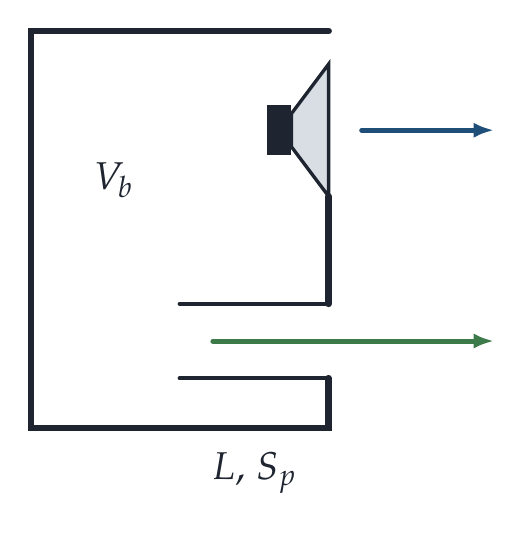
\begin{tikzpicture}[section]
    \draw[wall] (0,2.4) -- (-3.6,2.4) -- (-3.6,-2.4) -- (0,-2.4) -- (0,-1.8) (0,-0.9) -- (0,0.4);
    \driver{(0,1.2)}
    \draw[ink, line width=1.6pt] (0,-0.9) -- (-1.8,-0.9) (0,-1.8) -- (-1.8,-1.8);
    \draw[frontwave] (0.4,1.2) -- (2,1.2);
    \draw[portwave] (-1.4,-1.35) -- (2,-1.35);
    \node[lbl] at (-0.9,-2.95) {$L$, $S_p$};
    \node[lbl] at (-2.6,0.6) {$V_b$};
  \end{tikzpicture}}{%
  \begin{tikzpicture}
  \begin{semilogxaxis}[resp, xtick={1}, xticklabels={$f_b$}]
    \zerodb
    \addplot[muted, dashed, line width=1.2pt] {20*log10(hp(x/1.6,0.707))};
    \addplot[accent] {20*log10(x^4/sqrt(1+x^8))};
    \slope{0.13}{-30}{$-24$ dB/oct}
  \end{semilogxaxis}
  \end{tikzpicture}}
\impedance[xtick={1}, xticklabels={$f_b$}]{zpk(x,5,0.55,25)+zpk(x,5,1.8,25)}
\begin{eqgroup}[Helmholtz: the port's air mass on the box's air spring]
\[ f_b=\frac{c}{2\pi}\sqrt{\frac{S_p}{V_b\,L_\text{eff}}}\qquad L_\text{eff}\approx L+1.46\,r \]
\note{Thiele's B4: $Q_{ts}=0.383$, $V_b=0.707\,V_{as}$, $f_b=f_3=f_s$. Two peaks in $|Z|$; $f_b$ sits in the dip.}
\end{eqgroup}
\tcblower
\trap{\textbf{Below $f_b$ the cone is unloaded.} High-pass it, or it will leave the basket.}
\end{enclosure}
% ---------------------------------------------------------------- passive radiator
\begin{enclosure}[height=268mm, valign upper=center]{Passive radiator}{Put a cone where the port's air was.}%
  {Bluetooth and smart speakers, compact subwoofers.}
\figs{%
  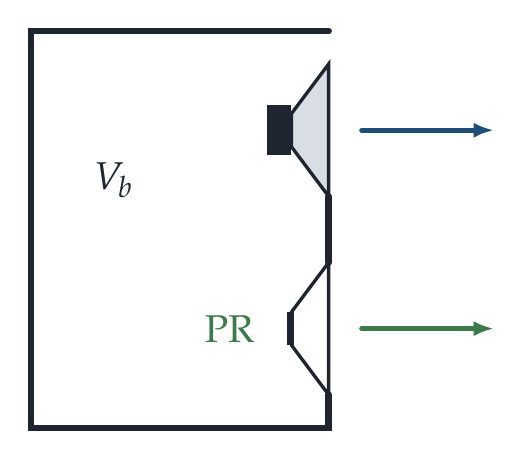
\begin{tikzpicture}[section]
    \draw[wall] (0,2.4) -- (-3.6,2.4) -- (-3.6,-2.4) -- (0,-2.4) -- (0,-2) (0,-0.4) -- (0,0.4);
    \driver{(0,1.2)}
    \radiator{(0,-1.2)}
    \draw[frontwave] (0.4,1.2) -- (2,1.2);
    \draw[portwave] (0.4,-1.2) -- (2,-1.2);
    \node[lbl] at (-2.6,0.6) {$V_b$};
    \node[lbl, text=good] at (-1.2,-1.2) {PR};
  \end{tikzpicture}}{%
  \begin{tikzpicture}
  \begin{semilogxaxis}[resp, xtick={0.5,1}, xticklabels={$f_p$,$f_b$}, samples=500]
    \zerodb
    \addplot[accent] {20*log10(x^4/sqrt(1+x^8)*abs(1-(0.5/x)^2))};
    \slope{1.3}{-30}{notch at $f_p$}
  \end{semilogxaxis}
  \end{tikzpicture}}
\impedance[xtick={1}, xticklabels={$f_b$}]{zpk(x,5,0.55,25)+zpk(x,5,1.8,25)}
\begin{eqgroup}[A port whose air has a suspension]
\[ f_p=\frac{1}{2\pi\sqrt{M_{mp}C_{mp}}}<f_b \]
\[ V_{d,\text{PR}}\ \ge\ (1.5\ldots2)\,V_d \]
\note{No port noise and no pipe resonances; below the notch the slope eases back to 12\,dB/oct.}
\end{eqgroup}
\tcblower
\trap{\textbf{The radiator must move more air than the woofer.} It is the larger cone, not the cheaper one.}
\end{enclosure}
% ---------------------------------------------------------------- bandpass
\begin{enclosure}[height=268mm, valign upper=center]{Bandpass}{Hide the driver; only the port speaks.}%
  {Car and PA subwoofers.}
\figs{%
  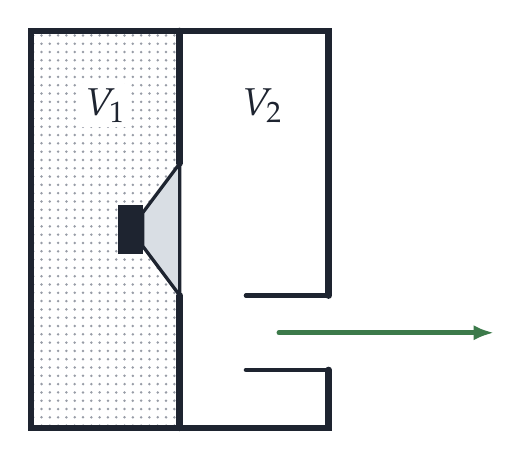
\begin{tikzpicture}[section]
    \fill[stuffing] (-3.6,-2.4) rectangle (-1.8,2.4);
    \draw[wall] (0,-0.8) -- (0,2.4) -- (-3.6,2.4) -- (-3.6,-2.4) -- (0,-2.4) -- (0,-1.7);
    \draw[wall] (-1.8,2.4) -- (-1.8,0.8) (-1.8,-0.8) -- (-1.8,-2.4);
    \driver{(-1.8,0)}
    \draw[ink, line width=1.6pt] (0,-0.8) -- (-1,-0.8) (0,-1.7) -- (-1,-1.7);
    \draw[portwave] (-0.6,-1.25) -- (2,-1.25);
    \node[lbl, fill=white, inner sep=1.5pt] at (-2.7,1.5) {$V_1$};
    \node[lbl] at (-0.8,1.5) {$V_2$};
  \end{tikzpicture}}{%
  \begin{tikzpicture}
  \begin{semilogxaxis}[resp, xtick={0.7,3}, xticklabels={$f_L$,$f_H$}]
    \zerodb
    \addplot[accent] {20*log10(hp(x/0.7,0.707)*lp(x/3,0.707))};
    \slope{0.12}{-30}{$-12$}
    \node[font=\small, text=muted, anchor=east] at (axis cs:9.5,-30) {$-12$};
  \end{semilogxaxis}
  \end{tikzpicture}}
\impedance[xtick={1}, xticklabels={$f_b$}]{zpk(x,5,0.6,25)+zpk(x,5,1.7,25)}
\begin{eqgroup}[Sealed rear chamber $V_1$, vented front chamber $V_2$]
\[ f_b=\frac{c}{2\pi}\sqrt{\frac{S_p}{V_2\,L_\text{eff}}} \]
\note{$V_1$ sets the low corner, the port and $V_2$ the high one. Narrow the band for gain, widen it for bandwidth; there is no third option.}
\end{eqgroup}
\tcblower
\trap{\textbf{Everything leaves through the port.} Port noise and pipe resonances are now the product.}
\end{enclosure}
% ---------------------------------------------------------------- transmission line
\begin{enclosure}[height=268mm, valign upper=center]{Transmission line}{Send the back wave down a long, damped pipe.}%
  {Some audiophile monitors.}
\figs{%
  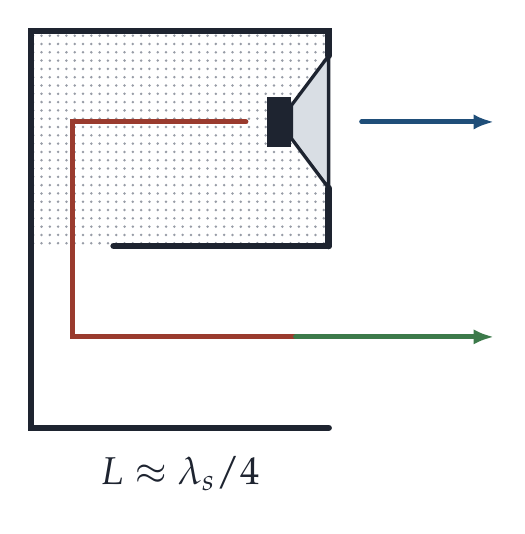
\begin{tikzpicture}[section]
    \fill[stuffing] (-3.6,-0.2) rectangle (0,2.4);
    \draw[wall] (0,-2.4) -- (-3.6,-2.4) -- (-3.6,2.4) -- (0,2.4) -- (0,2.1) (0,0.5) -- (0,-0.2);
    \draw[wall] (0,-0.2) -- (-2.6,-0.2);
    \driver{(0,1.3)}
    \draw[frontwave] (0.4,1.3) -- (2,1.3);
    \draw[backwave, -] (-1,1.3) -- (-3.1,1.3) -- (-3.1,-1.3) -- (-0.4,-1.3);
    \draw[portwave] (-0.4,-1.3) -- (2,-1.3);
    \node[lbl] at (-1.8,-2.95) {$L\approx\lambda_s/4$};
  \end{tikzpicture}}{%
  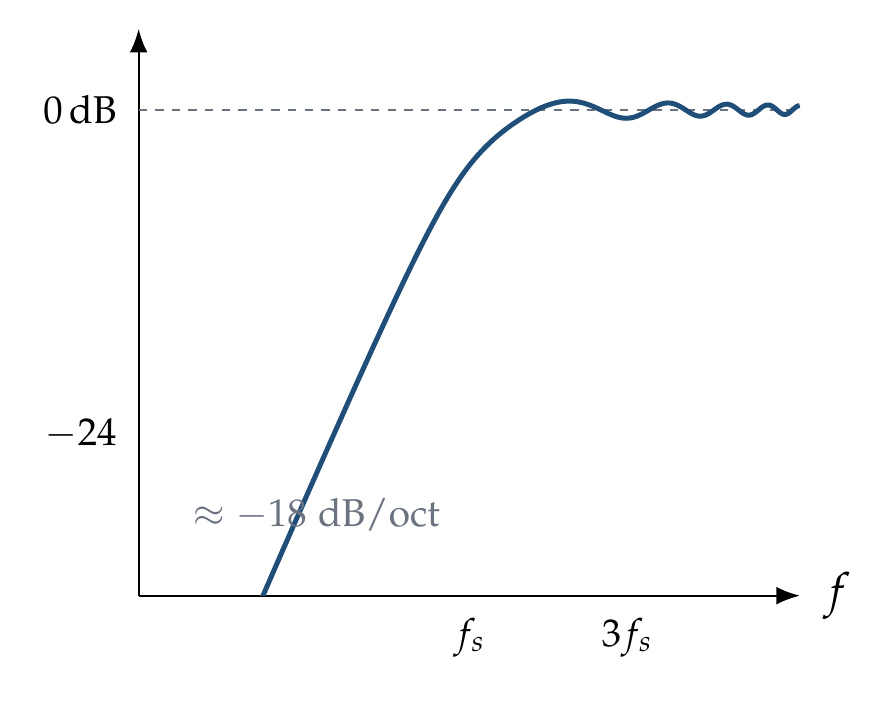
\begin{tikzpicture}
  \begin{semilogxaxis}[resp, xtick={1,3}, xticklabels={$f_s$,$3f_s$}]
    \zerodb
    \addplot[accent] {20*log10(x^3/sqrt(1+x^6)*(1+0.12*cos(deg(pi*x))/sqrt(x)))};
    \slope{0.13}{-30}{$\approx-18$ dB/oct}
  \end{semilogxaxis}
  \end{tikzpicture}}
\impedance[xtick={1,3}, xticklabels={$f_s$,$3f_s$}]{zpk(x,5,0.7,25)+zpk(x,3.5,1.45,25)+zpk(x,1.5,3.1,25)}
\begin{eqgroup}[A quarter-wave pipe, closed at the driver]
\[ L\approx\frac{c}{4f_s}\qquad\text{\small\color{muted}($f_s=35$\,Hz: 2.45\,m)} \]
\[ \text{resonances at } f_s,\ 3f_s,\ 5f_s,\ \ldots \]
\note{The stuffing absorbs the odd harmonics and slows the sound, so the real pipe is shorter.}
\end{eqgroup}
\tcblower
\trap{\textbf{An unstuffed pipe sings at $3f_s$ and $5f_s$.} Folded, it is also a carpentry exam.}
\end{enclosure}
% ---------------------------------------------------------------- horn
\begin{enclosure}[height=268mm, valign upper=center]{Horn}{Match the piston to the air.}%
  {PA and cinema, compression tweeters, the gramophone.}
\figs{%
  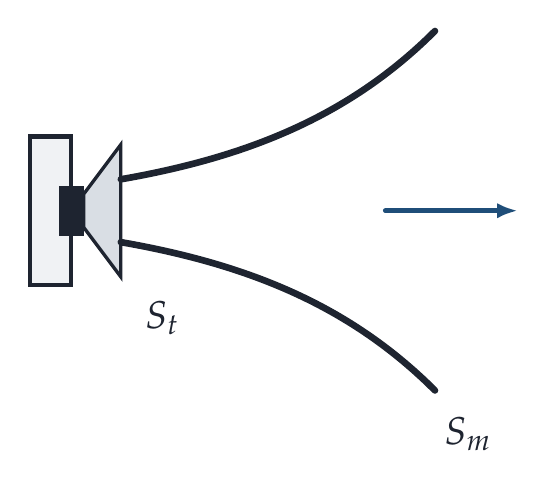
\begin{tikzpicture}[section]
    \draw[ink, line width=1.6pt, fill=steel!40] (-3.7,-0.9) rectangle (-3.2,0.9);
    \driver[0]{(-2.6,0)}
    \draw[wall] plot[domain=-2.6:1.2, samples=30, smooth] (\x,{0.38*exp(0.459*(\x+2.6))});
    \draw[wall] plot[domain=-2.6:1.2, samples=30, smooth] (\x,{-0.38*exp(0.459*(\x+2.6))});
    \draw[frontwave] (0.6,0) -- (2.2,0);
    \node[lbl] at (-2.1,-1.3) {$S_t$};
    \node[lbl] at (1.6,-2.7) {$S_m$};
  \end{tikzpicture}}{%
  \begin{tikzpicture}
  \begin{semilogxaxis}[resp, width=80mm, ymin=-24, ymax=16, ytick={0,10}, yticklabels={$0$\,dB,$+10$}, xtick={1}, xticklabels={$f_c$}]
    \zerodb
    \addplot[muted, dashed, line width=1.2pt] {20*log10(hp(x/0.5,0.707))};
    \addplot[accent, domain=1.0005:10] {10+10*log10(1-1/x^2)};
    \node[font=\small, text=muted, anchor=north east] at (axis cs:9.5,-3) {direct radiator};
  \end{semilogxaxis}
  \end{tikzpicture}}
\impedance[xtick={1}, xticklabels={$f_c$}]{zpk(x,2,0.6,4)}
\begin{eqgroup}[Exponential horn, $S(x)=S_t\,e^{mx}$]
\[ f_c=\frac{mc}{4\pi}\qquad R_t=\rho_0c\,S_t\sqrt{1-(f_c/f)^2} \]
\note{Efficiency 10--50\,\% against about 1\,\% for a cone in a box. The mouth needs a circumference of about $\lambda_c$.}
\end{eqgroup}
\tcblower
\trap{\textbf{At 50\,Hz the mouth is 2.2\,m across.} Bass horns are rooms, or use the room's corners.}
\end{enclosure}
\end{tcbraster}
\end{minipage}
\end{document}
